\chapter{Implementacja i testy na telefonie}

Ostatecznie zaimplementowano dwie wersje programu na urządzeniu mobilnym.
Pierwszy program był jednowątkowy, gdzie odczytany numer zapisywany
był tylko do pliku z~logami. Była
to wersja deweloperska i~nie zostały podjęte żadne próby optymalizacji
działania aplikacji. Celem przedsięwzięcia
było uruchomienie wszystkich komponentów na telefonie. Głównie
chodziło o~dostosowanie elementów aplikacji odpowiedzialnych za
dostęp do plików tekstowych i~graficznych zapisanych w~pamięci telefonu.
Był to obszar który najbardziej różnił aplikacje napisane z~myślą
o~uruchomienia na komputerze stacjonarnym od tych pisanych na telefon.

Druga wersja programu została wzbogacona o~komentarz głosowy
podczas jego działania. Wprowadzona została wielowątkowość, 
która powinna zwiększyć wydajność aplikacji uruchomionej na 
urządzeniu z~wieloma rdzeniami procesora.
Wprowadzona została minimalna funkcjonalność przepływu
sterowania aplikacją. Wprowadzone zostały dwa tryby wyszukiwania
i~tryb spoczynku. Jest to pierwsza wersja demonstracyjna, którą
bez dodatkowych modyfikacji można użyć do testów w~terenie.

\section{Pierwsza wersja programu - implementacja na dwuch urządzeniach}

Pierwszą wersję programu uruchomiono na dwóch urządzeniach:

\begin{itemize}
    \item HTC Desire Z,
    \item SONY Xperia E.
\end{itemize}

Na urządzeniu HTC osiągnięto wydajność rzędu 4-6 klatek na sekundę
w~trybie wyszukiwania frontu. Odnalezienie frontu i~przejście 
w~tryb odczytu numeru powodowało spadek częstotliwości odświeżania
do 0.76 klatki na sekundę (rysunek \ref{fig:imp_htc_v1}).

\begin{figure}[h!]
    \centering
    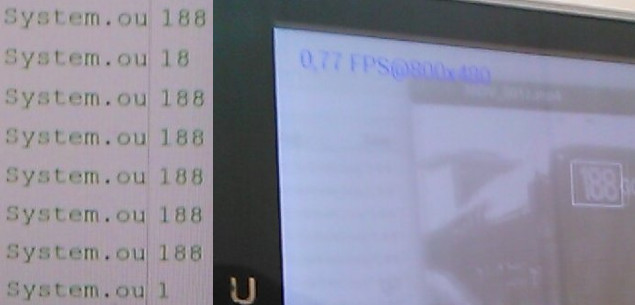
\includegraphics[width=0.9\textwidth]{img/imp_htc_v1}
    \caption{Wyniki pierwszej wersji programu na urządzeniu HTC}
    \label{fig:imp_htc_v1}
\end{figure}

Na urządzeniu SONY osiągnięto wydajność rzędu 6-8 klatek na sekundę
w~trybie wyszukiwania frontu. Odczyt numeru był na poziomie 0.97
klatki na sekundę (rysunek \ref{fig:imp_sony_v1}).

\begin{figure}[h!]
    \centering
    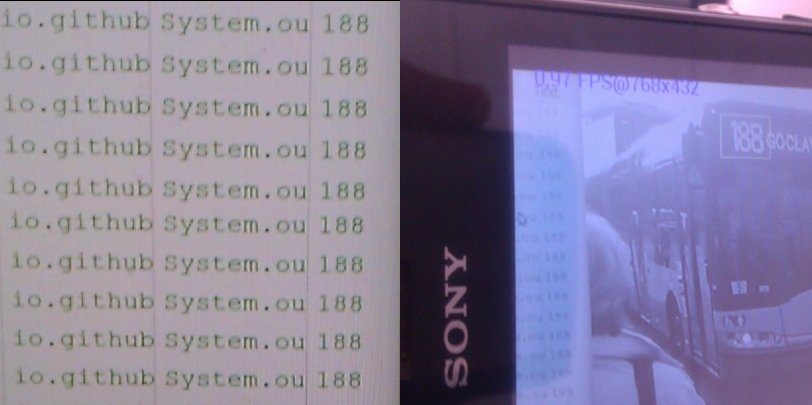
\includegraphics[width=0.9\textwidth]{img/imp_sony_v1}
    \caption{Wyniki pierwszej wersji programu na urządzeniu SONY}
    \label{fig:imp_sony_v1}
\end{figure}

Jak widać oba urządzenia są podobnej klasy. Ze względu na brak
znaczących różnic w~wydajności dalsze testy drugiej wersji 
programu odbywały się na urządzeniu SONY.

\section{Druga wersja programu}

Usprawnienia wprowadzone w~drugiej wersji miały na celu zwiększenie
wydajności, zwiększenie funkcjonalności oraz przystosowanie 
aplikacji do działań w~terenie.

Zwiększenie wydajności ograniczało się do doboru optymalnych parametrów
detektorów - funkcji \verb|detectMultiScale| - czyli:

\begin{itemize}
    \item współczynnika skalowania,
    \item minimalnych wymiarów czworokąta okalającego,
    \item maksymalnych wymiarów czworokąta okalającego,
    \item ilości sąsiadów.
\end{itemize}

Kluczowe dwa parametry to współczynnik skalowania i~minimalny rozmiar
obiektu. Dodatkowym czynnikiem wpływającym na wydajność było
skalowanie obrazu wejściowego. W~pierwszym kroku - detektor frontu -
klatka obrazu pobrana z~aparatu była zmniejszana do zadanej wartości
celem przyspieszenia procesu detekcji. Pozostałe kroki wykorzystywały
ten mechanizm raczej w~celu ujednolicenia wymiarów, czy to całych 
numerów czy pojedynczych cyfr. W~tabelce zamieszczono wszystkie 
parametry wykorzystane w~poszczególnych krokach.

\begin{table}[!h]
    \centering
    \begin{tabular}{r c c c c c }
        Etap    & Wysokość  & Wsp. skal.    & Min   & Max   & Sąsiedzi \\ \hline
        Front   & 140       & 1.02          & 60    & 120   & 10 \\
        Numer   & 150       & 1.01          & 30    & 150   & 5 \\
        Cyfry   & 110       & 1.01          & 40    & 110   & 40
    \end{tabular}
    \caption{Parametry detektorów}
    \label{tab:imp_det_params}
\end{table}

Funkcjonalność została zwiększona poprzez możliwość włączania i~wyłączania
trybu wyszukiwania. Dodany został komentarz słowny opisujący stany 
aplikacji. W~tym celu wykorzystano syntezator tekstu na mowę
obecny w~bibliotekach systemu android. W~wersji roboczej używane
były komunikaty w~języku angielski opisujące następujące stany:

\begin{itemize}
    \item po uruchomieniu aplikacji odczytywany był powitalny komunikat -
        ,,Point phone on bus front'',
    \item po wykryciu frontu aplikacja przechodziła w~stan zbierania
        maksymalnie stu klatek do bufora celem późniejszego przetworzenia.
        Towarzyszył temu zdarzeniu komunikat ,,Bus spotted, gathering
        data'',
    \item po zapełnieniu kolekcji (jeżeli odczyt nie nastąpił wcześniej),
        odczytywany był komunikat ,,Data gathered, processing'',
    \item opcjonalnie, gdy dla 20 klatek z~rzędu nie następowało wykrycie
        frontu następował odczyt komunikatu ,,Bus lost'', a~aplikacja
        automatycznie przechodziła w~stan spoczynku,
    \item ostatnim komunikatem był po prostu odczytany numer, po 
        odczytaniu tego komunikatu aplikacja również przechodziła
        w~stan spoczynku.
\end{itemize}

Zaimplementowany
mechanizm wielowątkowości zakładał istnienie trzech kolejek FIFO,
w~których umieszczano wyniki poszczególnych etapów algorytmu.
Po uruchomieniu aplikacja znajdowała się w~stanie spoczynku (idle)
i~dopiero po kliknięciu przycisku w~menu - Start/Stop - mogła
zostać wprowadzona w~stan wyszukiwania frontu w~scenie.
W~stanie wyszukiwania frontu uruchomiany był detektor frontów,
który przeszukiwał wszystkie pobrane z~aparatu klatki pod kątem
wystąpienia frontu autobusu. Po pierwszym odnalezieniu frontu
uruchamiane były wszystkie trzy wątki poprzez umieszczenie
stu kolejno pobranych obrazów do pierwszej kolejki.

Wątek główny umieszczał obrazy pobrane z~kamery telefonu do
pierwszej kolejki zawierającej pełne klatki. Proces ten trwał
do zapełnienia kolejki, której rozmiar określony był na 100 elementów.

Drugi wątek (pierwszy wątek tła) odpowiedzialny był za pobieranie 
obrazów z~pierwszej kolejki i~umieszczanie wycinków obrazów 
reprezentujących fronty
w~następnej kolejce. Wątek ten był uruchamiany wraz ze startem aplikacji
jednak gdy kolejka z~pełnymi klatkami była pusta, czy uległa właśnie 
wyczerpaniu, wątek wprowadzany był w~stan spoczynku i~sprawdzał co
100 ms czy kolejka ma elementy. W~podobny mechanizm wyposażony był
trzeci wątek. Tu z~kolei wejściowa kolejka zawierała fronty autobusów
na wyjściu natomiast uzupełniania była kolejka z~obrazami zawierającymi
jedynie numer linii.

Ostatni wątek - najbardziej intensywny obliczeniowo - pobierał obrazy
z~kolejki z~numerami i~kolejno uruchamiał detektory cyfr oraz 
funkcję dopasowującą wzorce. Wynikiem pojedynczej iteracji był 
ciąg znaków zawierający odczytany numer. Pewnego rodzaju zabezpieczeniem
było umieszczanie odczytanych ciągów znaków w~słowniku z~przypisaną
im liczbą wystąpień. Po osiągnięciu pewnej z~góry zadanej liczby
odczytów wybierany był ten numer do którego przypisana była największa 
liczba wystąpień. Wtedy automat odczytywał numer i~wprowadzał 
aplikację w~stan jałowy.

Przykładowy film z~działania aplikacji można znaleźć na kanale
,,Kuba Sałkowski'' w~serwisie YouTube. Można tam również znaleźć 
większość z~pozostałych przeprowadzonych eksperymentów.

Na zakończenie wykonano dziesięć prób wykrycia numeru autobusu
ze statycznego zdjęcia wyświetlanego na ekranie monitora.
Zdjęcie przedstawiało autobus Neoplan linii 188 jak na rysunku poniżej.

\begin{figure}[h!]
    \centering
    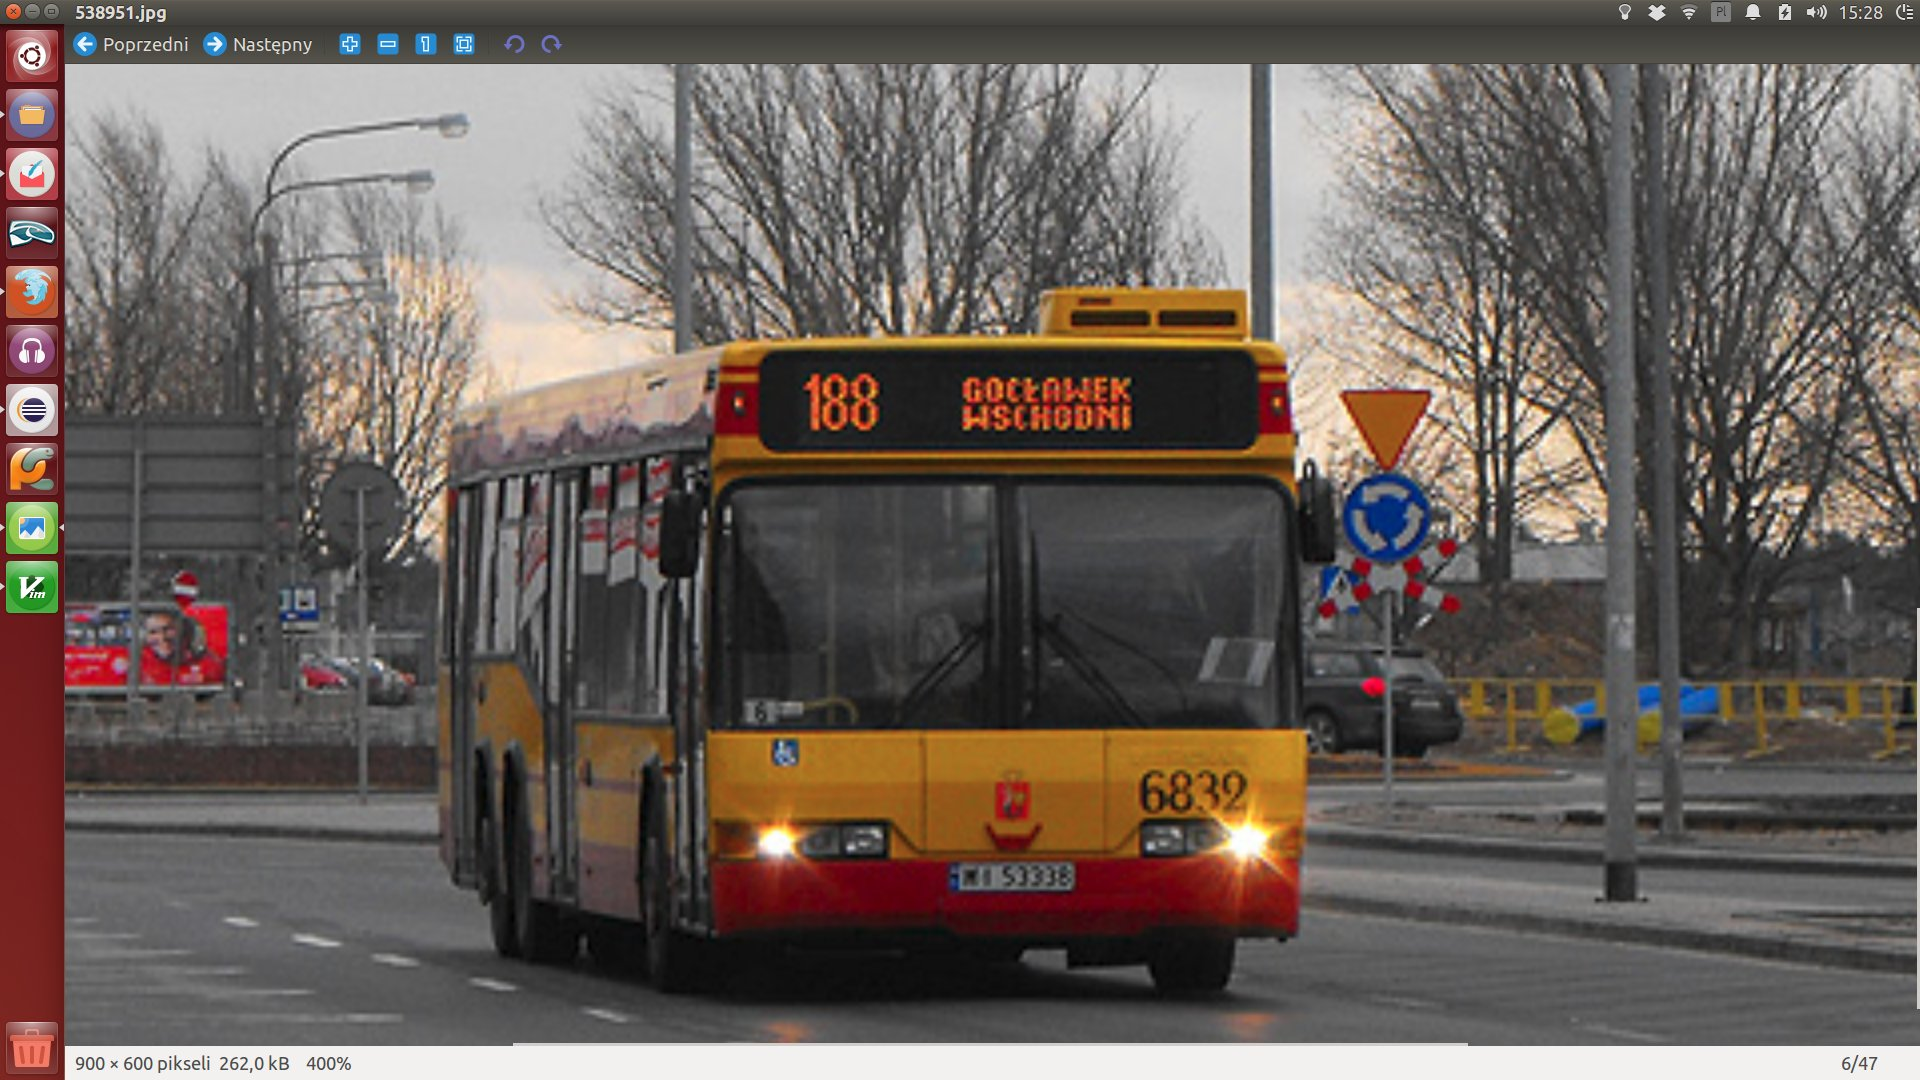
\includegraphics[width=0.9\textwidth]{img/imp_final_test_img}
    \caption{Obraz testowy ostatecznej wersji programu}
\end{figure}

Dla przedstawionego zdjęcia otrzymano wyniki zaprezentowane
w~tabeli \ref{tab:imp_lab_final_test_result}.

\begin{table}[!h]
    \centering
    \begin{tabular}{r c c c l }
        Lp. & Zebranie 100 próbek   & Odczyt    & Suma  & Wynik \\ \hline
        1   & 06.72                 & 07.03     & 13.75 & 188   \\
        2   & 06.57                 & 02.84     & 09.41 & 18    \\
        3   & 05.35                 & 04.36     & 09.71 & 188   \\
        4   & 05.65                 & 10.90     & 16.55 & Error \\
        5   & 06.30                 & 04.05     & 10.35 & 166   \\
        6   & 05.90                 & 07.36     & 13.26 & 188   \\
        7   & 06.04                 & 04.99     & 11.03 & 188   \\
        8   & 06.35                 & 02.86     & 09.21 & 1     \\
        9   & 05.60                 & 05.95     & 11.55 & 188   \\
        10  & 05.15                 & 07.38     & 12.53 & 188   \\
    \end{tabular}
    \caption{Wyniki testów manualnych w~warunkach laboratoryjnych}
    \label{tab:imp_lab_final_test_result}
\end{table}

Podsumowując, średni czas potrzebny na zebranie 100 próbek to około 6
sekund. Trudno określić czas potrzebny na odczyt, ponieważ 
wątek odpowiedzialny za to zadanie uruchamiany był zaraz 
po zebraniu i~wyłuskaniu obszaru z~numerem z~pierwszej klatki 
zawierającej front autobusu. Jednak widać, że ilość uruchomionych
detektorów miała duży wpływ na długość tej fazy. Cechowała się
ona też dużą zmiennością - od 3 do 11 sekund. Co prawda czas 
poniżej 3 sekund osiągnięto dla próby w~której otrzymano wynik błędny,
a~czas powyżej 10 sekund był wynikiem błędu aplikacji. 
Dla poprawnych rezultatów czasy wahały się od 4 do 7 sekund.

Czas od rozpoznania pierwszego wystąpienia
frontu do pełnego wyhamowania autobusu to od 3 do 5 sekund. Faza zbierania 
pełnych klatek wydaje się więc być jednym z~pierwszych elementów 
w~kolejce do usprawnienia. Kryterium końcowym fazy pobierania obrazów
mogło by być osiągnięcie przez kwadrat okalający odpowiedniej 
zadanej z~góry maksymalnej wysokości lub wielkość w~ogóle. 
Jasnym jest, że końcowa wersja programu przygotowana na potrzeby
tego opracowania jest dopiero punktem wyjścia do dalszych 
bardziej niezawodnych implementacji. Wydaje się, że wiele usprawnień
można wprowadzić niewielkim nakładem pracy. Niestety 
do osiągnięcia zadowalających wyników niezbędnym jest wprowadzenie
ich niemal w~każdej fazie algorytmu i~elemencie programu. 
Ważnym aspektem pozostaje weryfikacja dokładności i~skuteczności
działania algorytmu o~czym szerzej w~podsumowaniu.

